\nonstopmode
\documentclass{article}

\usepackage[utf8]{inputenc}
\usepackage{geometry}
\usepackage{graphicx}
\usepackage{polski}
\usepackage{subcaption}

\graphicspath{ {images/} }
\geometry{legalpaper, portrait, margin=1in}

\title{\LARGE Algorytmy z powracaniem\\ Sprawozdanie nr 4}
\author{Adam Piaseczny \\	151757 \and
				Igor Szczepaniak \\ 151918}
\date{Grupa piątkowa 11:45}

\begin{document}

\maketitle
\pagebreak

\tableofcontents
\pagebreak

\section{Wprowadzenie}

W tym sprawozdaniu zbadaliśmy znaczenie gęstości przy wyznaczaniu cykli Hamiltona oraz cyklu Eulera w grafach nieskierowanych. Kod źródłowy został napisany w języku \textbf{python} ze względu na prostotę implementacji.

Wygenerowaliśmy 15 losowych grafów nieskierowanych $G=(V,E)$ o rożnych $|V|=n$ posiadających cykl Hamiltona oraz Eulera. Dla każdego pomiaru czasowego uśredniliśmy wyniki z 3 przebiegów programu.

\section{Wstęp teoretyczny}

Droga Eulera to ścieżka w grafie, która przechodzi przez każdą jego krawędź dokładnie raz. Jeśli droga Eulera zaczyna się i kończy na tym samym wierzchołku, stanowi cykl Eulera. Warunkiem koniecznym i dostatecznym istnienia cyklu Eulera jest parzystość stopnia wszystkich wierzchołków oraz spójność grafu. Dla każdego grafu zmierzyliśmy ilość czasu potrzebną na znalezienie cyklu Eulera dla danego $n$, czas ten będzie oznaczony jako $t_E$.  Sprawdzanie istnienia cyklu Eulera w grafie może być osiągnięte następującym algorytmem:

\begin{itemize}
	\item algorytm drogaEulera($V$):
	\item Iterujemy przez wszystkie krawędzie $E$ wychodzące z wierzchołka $V$
	\begin{enumerate}
		\item Uruchamiamy drogaEulera dla wierzchołka sąsiądujego z $V$ po krawędzi $E$
		\item Usuwamy krawędź $E$ z grafu
	\end{enumerate}
	\item Dodajemy V do rozwiązania
\end{itemize}

Algorytm ten ma złożoność $O(m)$ i zależy od liczby krawędzi $m=\frac{d}{2}\times n \times (n-1)$, gdzie $d$ jest gęstością grafu. Złożoność wynika z faktu odwiedzenia każdej krawędzi w grafie dokładnie raz oraz usuwania odwiedzonej krawędzi w stałym czasie. Dodatkowo do całkowitego czasu wykonania algorytmu wlicza się również czas wyszukania kolejnej krawędzi $E$ wychodzącej z wierzchołka $V$, czas ten jest zależny od reprezentacji grafu co wyjaśniliśmy w dalszej części pracy.

Cykl Hamiltona to taki cykl w grafie, w którym każdy wierzchołek grafu odwiedzany jest dokładnie raz (oprócz pierwszego wierzchołka). Sprawdzenie czy graf posiada cykl Hamiltona opiera się na generowaniu permutacji kolejnych możliwych ścieżek z danego wierzchołka do nieodwiedzonych wierzchołków sąsiadujących. Posiadając wszystkie możliwe ścieżki możemy zweryfikować czy są one cyklami Hamiltona.

\section{Prezentacja wyników}

Czasy wyszukiwania pierwszego cyklu Eulera i Hamiltona w grafie oznaczyliśmy jako $t_E$ i $t_{H1}$, a wysuzkiwanie wszysktich cykli Hamiltona oznaczyliśmy jako $t_{HA}$. Poniższa tabela przedstawia wyniki dla gęstości grafu równej $d=0.6$.

\begin{figure}[h]
\centering
  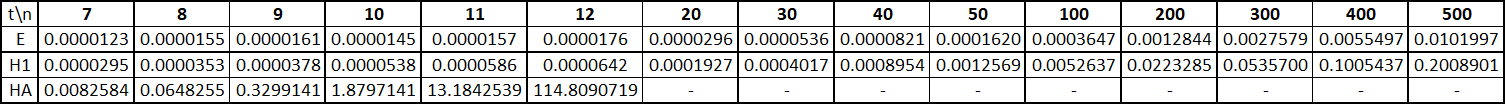
\includegraphics[width=1.0\linewidth]{zad2_tabela.png}
	\captionof{figure}{Prezentacja wyników - tabela}
\end{figure}%

Z wyników z stworzyliśmy następujący wykres:

\begin{figure}[h]
\centering
  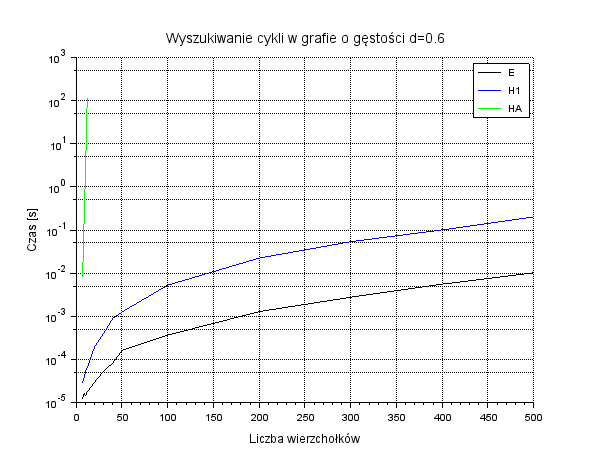
\includegraphics[width=0.5\linewidth]{zad2_wykres.png}
	\captionof{figure}{Prezentacja wyników}
\end{figure}%

Znajdywanie cyklu Eulera należy do problemów klasy P - jest to problem decyzyjny, gdzie rozwiązanie można znaleźć w czasie wielomianowym. Algorytm znajdywania cyklu Eulera opiera się na algorytmie DFS, który przebiega w czasie wielomianowym.

Do złożoności $O(m)$ algorytmu znajdywania cyklu Eulera należy dodać czas wyszukania kolejnej krawędzi. Lista sąsiadów jest odpowiednia dla tego zadania, gdyż może zwrócić kolejną krawędź w czasie $O(1)$ (przy usuwaniu odwiedzonych krawędzi w stałym czasie).

Znajdywanie cyklu Hamiltona jest problemem klasy silnie NP-zupełnych, co znaczy, że nie istnieje algorytm rozwiązujący ten problem w czasie wielomianowym; rozwiązanie problemu jest jednoznaczne ze znalezieniem takiego cyklu, lub wykazaniem jego braku. Ilość możliwych ścieżek w grafie wynosi $n!$, więc algorytm sprawdzający istnienie cykli Hamiltona ma złożoność $O(n!)$. Wraz ze wzrostem liczby wierzchołków $n$ czas wykonywania algorytmu drastycznie się zwiększa, przez co przebieg algorytmu dla większych wartości $n$ może okazać się nieopłacalne ze względu na czas wykonywania - z tego powodu przy wyszukiwaniu wszystkich cykli Hamiltona w grafie nie wykonywaliśmy testów dla wartości $n$ większej niż 12 ponieważ już dla 13 wierzchołków uznaliśmy czas działania algorytmu za zbyt długi. Złożoność algorytmu zarówno przy znajdywaniu pierwszego cyklu Hamiltona, jak i wszystkich istniejących w danym grafie, jest taka sama, ponieważ w najgorszym przypadku przy poszukiwaniu pierwszego cyklu Hamiltona wygerenujemy $(n-1)!$ permutacji.

\end{document}
